\documentclass[../../main]{subfiles}

\begin{document}
\chapter{補間多項式}
\label{chapter:interp}
\begin{lead}
補間多項式は,与えられた点を通る次数最小の多項式である.
補間多項式はそれ自身が有用であるだけでなく,数値微分や数値積分など,数値計算の様々な手法を基礎づける.
\cref{chapter:interp}では補間多項式を定義し,近似の観点からその性質を調べていく.
\end{lead}

\section{ラグランジュ補間}
\label{section:lagrange}
\cref{subsection:lagrange}の目的は,与えられた点を通る多項式関数を計算する方法である「ラグランジュ補間」を示すことである.

\label{subsection:lagrange}
\begin{theorem}{補間多項式の一意存在性}{interp}
\(xy\)平面上の点\(P_1=(p_1,q_1),\dots,P_n=(p_n,q_n)\)は,どの2点も\(x\)座標を共有しないとする.
このとき,\(f(p_i)=q_i\)(\(i=1,\dots,n\))を満たす次数が\(n-1\)以下の多項式\(f(x)\in\polyset{\numset{R}}{x}\)が一意に存在する.
\end{theorem}

\begin{proof}
まず,\(f(x)\)が存在することを示す.\(g_i(x)=\prod_{k\neq i}(x-p_k)\)とおく.
このとき\(g_i(p_i)\neq 0\)なので,\(f(x)=\sum_{i=1}^n(q_i/g_i(p_i))g_i(x)\)で\(f(x)\)を定義できる.
各\(g_i(x)\)の次数は\(n-1\)以下なので,\(f(x)\)の次数も\(n-1\)以下である.
また,\(i\neq k\)なら\(g_i(p_k)=0\)だから
\[
  f(p_k) = \sum_{i=1}^n\frac{q_i}{g_i(p_i)}g_i(p_k)
  = \frac{q_k}{g_k(p_k)}g_k(p_k)
  = q_k\quad(k=1,\dots,n)
\]
となる.これで\(f(x)\)の存在は示せた.

次に,\(f(x)\)が一意であることを示す.\(f_1(x)\)と\(f_2(x)\)が\(f(x)\)の条件を満たせば,\(h(x)=f_1(x)-f_2(x)\)は\(h(p_i)=0\)を満たす.
よって,\(h(x)\)は各\(x-p_i\)で割りきれるから,\(h(x)=Q(x)(x-p_1)\dotsm(x-p_n)\)(\(Q(x)\in\polyset{\numset{R}}{x}\))と書ける.
\(h(x)\)の次数は\(n-1\)以下なので\(Q(x)=0\)であり,よって\(f_1(x)=f_2(x)\)である.
\end{proof}

\begin{definition}{補間多項式}{}
\cref{theorem:interp}の\(f(x)\)を,点\(P_1,\dots,P_n\)に関する\impact{補間多項式}\index{ほかんたこうしき@補間多項式}(interpolation polynomial)という.
\(f(x)\)は次のように表せる.
\begin{equation}
  \label{equation:lagrange}
  f(x) = \sum_{i=1}^nq_i\prod_{k\neq i}\frac{x-p_k}{p_i-p_k}  
\end{equation}
\end{definition}

なお,補間多項式を\cref{equation:lagrange}に基づいて得ることを\impact{ラグランジュ補間}\index{らぐらんじゅほかん@ラグランジュ補間}(Lagrange interpolation)という.
以降は「点\(P_1,\dots,P_n\)に関する補間多項式」と言ったとき,\impact{どの2点も\(x\)座標を共有しないことを仮定する}.

\begin{example}
\label{example:interp_1}
点\((1,4)\),\((3,0)\),\((4,1)\)に関する補間多項式は
\[
  f(x) = 4\cdot\frac{(x-3)(x-4)}{(1-3)(1-4)}+0\cdot\frac{(x-1)(x-4)}{(3-1)(3-4)}+1\cdot\frac{(x-1)(x-3)}{(4-1)(4-3)}
  = x^2-6x+9
\]
である.
\end{example}

\begin{example}
\label{example:interp_2}
点\((1,6)\),\((5,2)\),\((4,3)\)に関する補間多項式は
\[
  g(x) = 6\cdot\frac{(x-5)(x-4)}{(1-5)(1-4)}+2\cdot\frac{(x-1)(x-4)}{(5-1)(5-4)}+3\cdot\frac{(x-1)(x-5)}{(4-1)(4-5)}
  = -x+7
\]
である.このように,\(n\)個の点に関する補間多項式の次数は\(n-1\)になるとは限らない.
\end{example}

\begin{figure}[htbp]
  \centering
  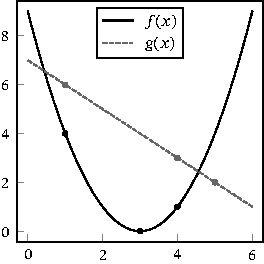
\includegraphics{interpolation.pdf}
  \caption{\cref{example:interp_1},\cref{example:interp_2}の補間多項式}
\end{figure}

\section{ニュートン補間}
\label{subsection:newton}
\cref{subsection:lagrange}では補間多項式を計算する方法として,\cref{equation:lagrange}に基づくラグランジュ補間を示した.
\cref{subsection:newton}では「ニュートン補間」という,補間多項式を計算するもう1つの方法を紹介する.

\begin{definition}{差商}{divided_difference}\index{\(\divdiff{P_1,\dots,P_n}\)}\index{\(\divdiff[f]{x_1,\dots,x_n}\)}
\(xy\)平面上の点\(P_1=(p_1,q_1),\dots,P_n=(p_n,q_n)\)は,どの2点も\(x\)座標を共有しないとする.
このとき,\(P_1,\dots,P_n\)の\impact{差商}\index{さしょう@差商}(divided differences)\(\divdiff{P_1,\dots,P_n}\)を次のように定義する\footnotemark .
\[
  \divdiff{P_1} = q_1,
  \quad\divdiff{P_1,\dots,P_n} = \frac{\divdiff{P_2,\dots,P_n}-\divdiff{P_1,\dots,P_{n-1}}}{p_n-p_1}\quad(n\geq 2)
\]
また,関数\(f\)が\(q_i=f(p_i)\)を満たすときは\(\divdiff{P_1,\dots,P_n}\)を\(\divdiff[f]{p_1,\dots,p_n}\)とも表記する.
\end{definition}
\footnotetext{多くの場合,差商は\(\divdiff{P_1,\dots,P_n}\)という形ではなく\([q_1,\dots,q_n]\)という形で表記されるのだが,\(\divdiff{P_1,\dots,P_n}\)が\(p_1,\dots,p_n\)に依存することを明示する目的で表記法を変えた.}

\begin{example}
\label{example:divdiff}
\(P_1=(1,4)\),\(P_2=(3,0)\),\(P_3=(4,1)\)のとき
\[
  \divdiff{P_1,P_2} = \frac{0-4}{3-1} = -2,
  \quad\divdiff{P_2,P_3} = \frac{1-0}{4-3} = 1,
  \quad\divdiff{P_1,P_2,P_3} = \frac{1-(-2)}{4-1} = 1
\]
である.
\end{example}

\begin{theorem}{ニュートン補間}{newton_interp}
点\(P_1=(p_1,q_1),\dots,P_n=(p_n,q_n)\)に関する補間多項式\(f(x)\)は次のように表せる.
\begin{equation}
  \label{equation:newton_interp}
  f(x) = q_1+\sum_{k=1}^{n-1}\divdiff{P_1,\dots,P_{k+1}}(x-p_1)\dotsm(x-p_k)
\end{equation}
\end{theorem}

\begin{proof}
点の個数に関する帰納法で示す.点の個数が\(n-1\)であるとき,\cref{equation:newton_interp}が成り立つと仮定する.
\(P_1,\dots,P_{n-1}\)に関する補間多項式を\(g(x)\),\(P_2,\dots,P_n\)に関する補間多項式を\(h(x)\)とおく.
このとき,多項式
\begin{equation}
  \label{equation:newton_proof}
  f(x) = \frac{(x-p_1)h(x)+(p_n-x)g(x)}{p_n-p_1}
  = \frac{(h(x)-g(x))x}{p_n-p_1}+\frac{p_ng(x)-p_1h(x)}{p_n-p_1}  
\end{equation}
は\(q_i=f(p_i)\)(\(i=1,\dots,n\))を満たす.また,\(g(x)\)と\(h(x)\)の次数は\(n-2\)以下だから,
\(f(x)\)の次数は\(n-1\)以下である.よって,\(f(x)\)は\(P_1,\dots,P_n\)に関する補間多項式である.
帰納法の仮定から,\(g(x)\)の\(n-2\)次の項は\(\divdiff{P_1,\dots,P_{n-1}}x^{n-2}\),\(h(x)\)の\(n-2\)次の項は\(\divdiff{P_2,\dots,P_n}x^{n-2}\)である.
よって\cref{equation:newton_proof}から,\(f(x)\)の\(n-1\)次の項は
\[
  \frac{\divdiff{P_2,\dots,P_n}-\divdiff{P_1,\dots,P_{n-1}}}{p_n-p_1}x^{n-1} = \divdiff{P_1,\dots,P_n}x^{n-1}
\]
である.

\(d(x)=f(x)-g(x)\)とおくと,\(d(p_i)=0\)(\(i=1,\dots,n-1\))であるから
\(d(x)\)は\(\prod_{i=1}^{n-1}(x-p_i)\)で割り切れる.この商を\(Q(x)\)とすると,
\(d(x)\)は\(Q(x)\prod_{i=1}^{n-1}(x-p_i)\)と書ける.

\(f(x)\),\(g(x)\)の次数は\(n-1\)以下なので,\(d(x)\)の次数も\(n-1\)以下である.よって,\(Q(x)\)は定数である.
\(Q(x)=c\)とおくと
\[
  f(x) = g(x)+c\prod_{i=1}^{n-1}(x-p_i)
  = \pqty*{q_1+\sum_{k=1}^{n-2}\divdiff{P_1,\dots,P_{k+1}}\prod_{i=1}^k(x-p_i)}+c\prod_{i=1}^{n-1}(x-p_i)
\]
であり,右辺の\(n-1\)次の項は\(cx^{n-1}\)だから\(c=\divdiff{P_1,\dots,P_n}x^{n-1}\)である.
よって,\cref{equation:newton_interp}は点の個数が\(n\)であるときも成立する.
\end{proof}

補間多項式を\cref{equation:newton_interp}に基づいて得ることを\impact{ニュートン補間}\index{にゅーとんほかん@ニュートン補間}(Newton interpolation)という.
ラグランジュ補間とニュートン補間で計算結果は変わらないが,ニュートン補間を使うと計算しやすくなる場合がある.
たとえば,\(P_1,\dots,P_{n-1}\)に関する補間多項式\(f_{n-1}(x)\)が計算済みであるとき,\(P_1,\dots,P_n\)に関する補間多項式\(f_n(x)\)を計算するには,
\(\divdiff{P_1,\dots,P_n}(x-p_1)\dotsm(x-p_{n-1})\)を計算して\(f_{n-1}(x)\)に足せばよい.

\begin{example}
\cref{example:divdiff}から,\(P_1\),\(P_2\),\(P_3\)に関する補間多項式は
\(4+(-2)(x-1)+1(x-1)(x-3)=x^2-6x+9\)である.\nameref{theorem:interp}からも分かるように,これは\cref{example:interp_1}の多項式と一致している.
\end{example}

\section{補間多項式による近似の誤差}
\(n\)を\(2\)以上の整数とする.\(f\)を関数とし,点\(P_1=(x_1,f(x_1)),\dots,P_n=(x_n,f(x_n))\)(\(x_1<\dots<x_n\))に関する補間多項式を\(p(x)\)とおく.
このとき,\(f\)が十分に滑らかであれば,\(x\)が\(x_1,\dots,x_n\)に近いとき\(f(x)\)の値と\(p(x)\)の値はごく近いことが期待できる.
次の定理はこのことを保証するものである.

\begin{theorem}{補間多項式による近似の誤差評価式}{interp_error}
上の状況で\(f\)が\(\ccival{x_1}{x_n}\)で連続,\(\ooival{x_1}{x_n}\)で\(n\)階微分可能なら,任意の\(t\in\ooival{x_1}{x_n}\)に対して\(\xi\in\ooival{x_1}{x_n}\)が存在し
\begin{equation}
  \label{equation:interp_error}
  f(t)-p(t) = \frac{f^{(n)}(\xi)}{n!}(t-x_1)\dotsm(t-x_n)  
\end{equation}
を満たす.このことから,\(f^{(n)}(x)\)が区間\(\ccival{x_1}{x_n}\)で最大値に達するとき,次の不等式が成立する.
\[
  \abs{f(t)-p(t)} \leq \max_{\xi\in\ccival{x_1}{x_n}}\frac{\abs{f^{(n)}(\xi)}}{n!}\prod_{i=1}^n\abs{t-x_i}
  \leq \max_{\xi\in\ccival{x_1}{x_n}}\frac{\abs{f^{(n)}(\xi)}}{n!}(x_n-x_1)^n
\]
\end{theorem}

\cref{theorem:interp_error}を示すために,次の補題を用意する.

\begin{lemma}{}{zero_existance}
関数\(g\)は\(\ccival{a}{b}\)(\(-\infty<a<b<\infty\))で連続,\(\ooival{a}{b}\)で\(n\)階微分可能であるとする.
このとき,\(g(x)=0\)を満たす\(x\in\ccival{a}{b}\)が\(n+1\)個あれば,\(g^{(n)}(\xi)=0\)を満たす\(\xi\in\ooival{a}{b}\)が存在する.
\end{lemma}

\begin{proof}
帰納法で示す.\(n=k-1\)のとき\cref{lemma:zero_existance}が成り立つと仮定する.
\(g\)は\(\ooival{a}{b}\)で\(k\)階微分可能とする.また,\(x_1,\dots,x_{k+1}\in\ccival{a}{b}\)は\(x_1<\dots<x_{k+1}\),\(g(x_1)=\dots=g(x_{k+1})=0\)を満たすとする.
このときロルの定理から,各\(i=1,\dots,k\)に対して\(\xi_i\in\ooival{x_i}{x_{i+1}}\)が存在し\(g'(\xi_i)=0\)を満たす.
\(a'=(a+\xi_1)/2\),\(b'=(\xi_k+b)/2\)とおくと,関数\(g'\)は\(\ccival{a'}{b'}\)で連続,\(\ooival{a'}{b'}\)で\(k-1\)階微分可能である.
よって,帰納法の仮定から\((\diff*[k-1]{g'}/{x})(\xi)=g^{(k)}(\xi)=0\)を満たす\(\xi\in\ooival{a'}{b'}\)が存在する.
したがって,\cref{lemma:zero_existance}は\(n=k\)のときも成立する.
\end{proof}

これで準備はできた.\cref{theorem:interp_error}を示そう.

\begin{proof}[\cref{theorem:interp_error}の\proofname]
\(t=x_1,\dots,x_n\)のときは明らかに成り立つので,\(t\notin\Set{x_1,\dots,x_n}\)のときについて示す.
\[
  g(x) = f(x)-p(x)-(f(t)-p(t))\frac{\prod_{i=1}^n(x-x_i)}{\prod_{i=1}^n(t-x_i)}
\]
とおくと,関数\(g\)は\(n\)階微分可能かつ,\(g(t)=g(x_1)=\dots=g(x_n)=0\)である.よって,\cref{lemma:zero_existance}から
\(g^{(n)}(\xi)=0\)を満たす\(\xi\in\ooival{x_1}{x_n}\)が存在する.\(p(x)\)の次数は\(n-1\)以下なので\(p^{(n)}(x)=0\)である.したがって
\begin{align*}
  g^{(n)}(x) &= f^{(n)}(x)-(f(t)-p(t))\frac{1}{\prod_{i=1}^n(t-x_i)}\diff*[n]{\prod_{i=1}^n(x-x_i)}{x} \\
  &= f^{(n)}(x)-(f(t)-p(t))\frac{n!}{\prod_{i=1}^n(t-x_i)}
\end{align*}
であり,\(x=\xi\)とすると\cref{equation:interp_error}が得られる.
\end{proof}

\begin{example}
\(\sin\degree{10.5}\)の近似値を求めよう.数表から,近似値
\[
  \sin\degree{10} = 0.1736,
  \quad\sin\degree{11} = 0.1908,
  \quad\sin\degree{12} = 0.2079
\]
が分かっているとする.このとき,点\((10,0.1736)\),\((11,0.1908)\),\((12,0.2079)\)に関する補間多項式は\(p(x)=-0.00005x^2+0.01825x-0.0039\)
であるから,\(\sin\degree{10.5}\)の近似値は\(\sin\degree{10.5}\fallingdotseq p(10.5)=0.182213\)となる.

\begin{figure}[htbp]
  \centering
  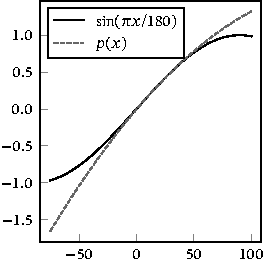
\includegraphics{sin.pdf}
  \caption{\(\sin(\krez x/180)\)と\(p(x)\)の比較}
\end{figure}

この近似の妥当性を考える.\cref{theorem:interp_error}と
\[
  \abs*{\diff*[3]{\sin\pqty*{\frac{\krez}{180}x}}{x}} = \abs*{\pqty*{\frac{\krez}{180}}^3\cos\pqty*{\frac{\krez}{180}x}}
  \leq \pqty*{\frac{\krez}{180}}^3
\]
から
\[
  \abs*{\sin\degree{10.5}-p(10.5)} \leq \pqty*{\frac{\krez}{180}}^3\frac{1}{3!}\abs{12-10}^3
  \fallingdotseq 7.08\times 10^{-6}
\]
である.これは利用した近似値の有効数字である4桁よりも十分に小さいので,\(\sin\degree{10.5}=0.1822\)は有効数字4桁で正しいと考えられる
(実際\(\sin\degree{10.5}=0.182236\dots\)なので,確かに有効数字4桁で正しい値が得られている).
また,有効数字4桁の数表に基づく限り,補間多項式の次数をこれ以上増やす必要は無いことも分かる.
\end{example}

\section{補間多項式とテイラー多項式の関係}
\label{section:taylor}
\cref{section:taylor}では,補間多項式がテイラー多項式\(T_n(x)=\sum_{k=0}^nf^{(k)}(t)(x-t)^k/k!\)
の近似と見なせることを示す.

まず\(n=2\)のときについて考える.2次のテイラー多項式
\[
  T_2(x) = f(t)+f'(t)(x-t)+\frac{f''(t)}{2}(x-t)^2
\]
について,この式に表れる微分係数を
\[
  f'(t) \fallingdotseq \frac{f(t+h)-f(t)}{h},
  \quad f''(t) \fallingdotseq \frac{(f(t+h)-f(t))/h-(f(t)-f(t-h))/h}{h}
\]
のように,微小な正数\(h\)を用いて近似する.この近似は次のように書き換えられる.
\[
  f'(t) \fallingdotseq \divdiff[f]{t+h,t},
  \quad f''(t) \fallingdotseq 2\cdot\frac{\divdiff[f]{t+h,t}-\divdiff[f]{t,t-h}}{(t+h)-(t-h)}
  = 2\divdiff[f]{t+h,t,t-h}
\]

すると,これを\(T_2(x)\)に代入すれば
\[
  T_2(x)\fallingdotseq f(t)+\divdiff[f]{t,t-h}(x-t)+\divdiff[f]{t+h,t,t-h}(x-t)^2
\]
となり,さらに,\(\abs{h}\)の値が十分小さければ\(x-(t+h)\fallingdotseq x-t\)なので
\[
  T_2(x)\fallingdotseq f(t)+\divdiff[f]{t+h,t}(x-(t+h))+\divdiff[f]{t+h,t,t-h}(x-(t+h))(x-t)
\]
である.\cref{theorem:newton_interp}から,右辺は点\((t-h,f(t-h))\),\((t,f(t))\),\((t+h,f(t+h))\)に関する補間多項式である.

以下では一般の\(n\)についても,補間多項式がテイラー多項式の近似と見なせることを示す.

\begin{theorem}{差商に対する平均値の定理}{divdif_mean}
実数\(x_1,\dots,x_{n+1}\)はどの2つも相異なるとし,\(x_1,\dots,x_{n+1}\)の中で最小のものを\(m\),最大のものを\(M\)とおく.
また,関数\(f\)は区間\(\ccival{m}{M}\)で連続,\(\ooival{m}{M}\)で\(n\)階微分可能であるとする.
このとき,次式を満たす\(\xi\in\ooival{m}{M}\)が存在する.
\[
  \divdiff[f]{x_1,\dots,x_{n+1}} = \frac{f^{(n)}(\xi)}{n!}
\]
\end{theorem}

\begin{proof}
点\((x_1,f(x_1)),\dots,(x_{n+1},f(x_{n+1}))\)に関する補間多項式を\(p(x)\)とおくと,
関数\(g(x)=f(x)-p(x)\)は\(x_1,\dots,x_{n+1}\)を零点に持つ.
したがって,\cref{lemma:zero_existance}から\(g^{(n)}(\xi)=0\)を満たす\(\xi\in\ooival{m}{M}\)が存在する.
\cref{theorem:newton_interp}より
\[
  p(x) = f(x_1)+\sum_{k=1}^{n}\divdiff[f]{x_1,\dots,x_{k+1}}(x-x_1)\dotsm(x-x_k)
\]
なので,\(p^{(n)}(x)=\divdiff[f]{x_1,\dots,x_{n+1}}n!\)である.
よって\(f^{(n)}(\xi)-\divdiff[f]{x_1,\dots,x_{n+1}}n!=0\)となる.
\end{proof}

議論を簡単にするために,標本点を等間隔にとって\(x_i=t+(i-1)h\)(\(h\neq 0\))とおく.
また,十分小さな\(\varepsilon>0\)に対して,関数\(f\)は\(\ccival{t-\varepsilon}{t+\varepsilon}\)を含むある開区間で\(n\)階微分可能かつ,
\(f\)の\(n\)次導関数は\(\ooival{t-\varepsilon}{t+\varepsilon}\)で連続であるとする.

点\((x_1,f(x_1)),\dots,(x_{n+1},f(x_{n+1}))\)に関する補間多項式\(p(x)\)は
\[
  p(x) = f(x_1)+\sum_{k=1}^n\divdiff[f]{x_1,\dots,x_{k+1}}(x-x_1)\dotsm(x-x_k)
\]
と書ける.ここで,\(h\)の値を\(\abs{h}<\varepsilon/n\)が成立するように十分小さくとる.このとき\(x_1,\dots,x_{n+1}\in\ccival{t-\varepsilon}{t+\varepsilon}\)なので,
\cref{theorem:divdif_mean}から各\(\divdiff[f]{x_1,\dots,x_{k+1}}\)に対して\(\xi_k\in\ooival{m}{M}\)(\(m=\min\Set{x_1,x_{n+1}}\),\(M=\max\Set{x_1,x_{n+1}}\))が存在し
\[
  \divdiff[f]{x_1,\dots,x_{k+1}} = \frac{f^{(k)}(\xi_k)}{k!}
\]
を満たす.また,\(m,M\to t\)(\(h\to 0\))より\(f^{(k)}(\xi_k)\to f^{(k)}(t)\)(\(h\to 0\))である.したがって
\begin{align*}
  p(x) &=f(x_1)+\sum_{k=1}^n\divdiff[f]{x_1,\dots,x_{k+1}}(x-x_1)\dotsm (x-x_k) \\
  &\to f(t)+\sum_{k=1}^n\frac{f^{(k)}(t)}{k!}(x-t)^k\quad(h\to 0)
\end{align*}
であり,右辺はテイラー多項式の形になっている.よって,標本点どうしの間隔が十分に狭ければ,補間多項式をテイラー多項式の近似と見なせる.

\section{数値微分}
関数を補間多項式で近似できるのなら,関数の微分係数もまた,補間多項式の微分係数で近似できると考えられる.
すなわち,\(t\)の値が\(x_1,\dots,x_n\)の値に十分近いとき,点\((x_1,f(x_1)),\dots,(x_n,f(x_n))\)に関する補間多項式を\(p_n(x)\)とすると\(f'(t)\fallingdotseq\eval{p_n'(x)}_{x=t}\)であると期待できる.

このような微分の近似を\impact{数値微分}\index{すうちびぶん@数値微分}(numerical differentiation)という.数値微分をするときは\(x_1,\dots,x_n\)を等間隔に取ることが多い.以下にこの場合の例を示す.

\begin{example}
\label{example:numerical_differentiation_1}
\((x_1,x_2)=(t,t+h)\)のとき\(p_2(x)=f(t)+\divdiff[f]{t,t+h}(x-t)\)である.よって,\(p_2(x)\)に基づく\(f\)の数値微分は
\[
  f'(t) \fallingdotseq \eval{p_2'(x)}_{x=t}
  = \divdiff[f]{t,t+h}
  = \frac{f(t+h)-f(t)}{h}
\]
となる.\(h\to 0\)では,右辺は厳密に\(f'(t)\)と等しくなる.
\end{example}

\begin{example}
\label{example:numerical_differentiation_2}
\((x_1,x_2,x_3)=(t-h,t,t+h)\)のとき
\[
  p_3(x) = f(t-h)+\divdiff[f]{t-h,t}\pqty*{x-(t-h)}+\divdiff[f]{t-h,t,t+h}\pqty*{x-(t-h)}(x-t)
\]
である.よって,\(p_3(x)\)に基づく\(f\)の数値微分は
\begin{align*}
  f'(t) &\fallingdotseq \eval{p_3'(x)}_{x=t} = \divdiff[f]{t-h,t}+\divdiff[f]{t-h,t,t+h}h \\
  &= \frac{f(t)-f(t-h)}{h}+\frac{(f(t+h)-f(t))/h-(f(t)-f(t-h))/h}{(t+h)-(t-h)}h \\
  &= \frac{f(t+h)-f(t-h)}{2h}  
\end{align*}
となる.この式についても,\(h\to 0\)では
\[
  \frac{f(t+h)-f(t-h)}{2h} = \frac{f(t+h)-f(t)}{2h}+\frac{f(t)-f(t-h)}{2h}
  \to f'(t)\quad(h\to 0)
\]
が成立する.
\end{example}

\begin{figure}[htbp]
  \centering
  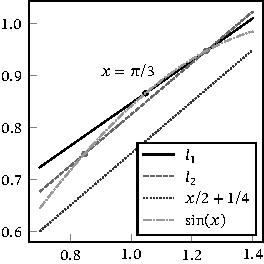
\includegraphics{differentiation.pdf}
  \caption{数値微分の比較}
  \label{figure:differentiation}
\end{figure}

\cref{figure:differentiation}は,2つの直線
\begin{align*}
  l_1 &\colon y=\frac{f(t+h)-f(t)}{h}(x-t)+f(t), \\
  l_2 &\colon y=\frac{f(t+h)-f(t-h)}{2h}(x-(t-h))+f(t-h)
\end{align*}
を\(f(x)=\sin(x)\),\(t=\krez/3\),\(h=0.2\)の場合について示したものである.
\cref{figure:differentiation}によれば,\(l_2\)は\(l_1\)よりも傾きが\(1/2=\cos(\krez/3)\)に近い.
したがって,\((\sin(x))'\)の\(x=\krez/3\)における近似に関しては,\cref{example:numerical_differentiation_1}の近似よりも\cref{example:numerical_differentiation_2}の近似のほうが,真値に近い値を与えている.

\cref{example:numerical_differentiation_1}の近似と\cref{example:numerical_differentiation_2}の近似をより数学的に比較するために,次の記法を定義する.

\begin{definition}{ランダウの記号}{landau-notation}\index{\(f(x)=\Order(g(x))\)}
関数\(f\),\(g\)は実数\(a\)の周りで定義されているとする.正数\(\delta\),\(C\)が存在して「\(0<\abs{x-a}<\delta\implies\abs{f(x)}\leq C\abs{g(x)}\)」が成り立つとき
\[
  f(x) = \Order(g(x))\quad(x\to a)
\]
と書く.この記法を\impact{ランダウの記号}\index{らんだうのきごう@ランダウの記号}(Big O notation)という.
また,\(a\)の値が文脈から明らかなときは\(f(x)=\Order(g(x))\)とも表記する.
\end{definition}

\begin{example}
\label{example:bigo_ratio}
関数\(f\),\(g\)は実数\(a\)の周りで定義され,ある\(\varepsilon>0\)に対し
\[
  g(x)\neq 0\quad(0<\abs{x-a}<\varepsilon)
\]
であるとする.このとき,極限値\(\lim_{x\to a}\abs{f(x)/g(x)}\)が存在して有限なら\(f(x)=\Order(g(x))\)(\(x\to a\))である.
実際\(\abs{f(x)/g(x)}\to\alpha\)(\(x\to a\))なら,\(C>0\)と\(\delta\in\ooival{0}{\varepsilon}\)の組で「\(\abs{x-a}<\delta\implies\abs{\abs{f(x)/g(x)}-\alpha}<C\)」を満たすものが存在する.
よって,\(\abs{x-a}<\delta\)なら
\[
  \abs*{\frac{f(x)}{g(x)}} = \abs*{\abs*{\frac{f(x)}{g(x)}}-\alpha+\alpha}
  \leq \abs*{\abs*{\frac{f(x)}{g(x)}}-\alpha}+\alpha
  < C+\alpha
\]
だから\(\abs{f(x)}\leq(C+\alpha)\abs{g(x)}\)である.したがって\(f(x)=\Order(g(x))\)が成立する.

一方,\(x\neq 0\)のとき\(f(x)=x\sin(1/x)\),\(x=0\)のとき\(f(x)=0\)とおくと,\(\abs{f(x)}\leq\abs{x}\)なので\(f(x)=\Order(x)\)(\(x\to 0\))だが,
\(\abs{f(x)/x}=\abs{\sin(1/x)}\)は原点付近で激しく振動するから,極限値\(\lim_{x\to 0}\abs{f(x)/x}\)は存在しない.
\end{example}

\begin{figure}[htbp]
  \begin{minipage}{0.5\linewidth}
    \centering
    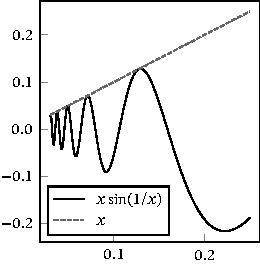
\includegraphics{asymptotic.pdf}
    \caption{\(x\sin(1/x)\)のグラフ}
  \end{minipage}%
  \begin{minipage}{0.5\linewidth}
    \centering
    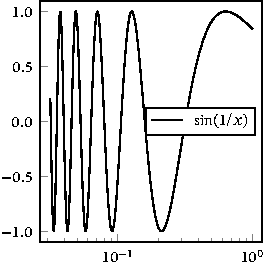
\includegraphics{nolimits.pdf}
    \caption{\(\sin(1/x)\)の片対数グラフ}
  \end{minipage}
\end{figure}

なお,ランダウの記号が両辺に複数回表れるときは,式の意味を以下の通り定義する.
任意の関数\(f\)に対し,関数の集合\([f]\)を\([f]=\Set{\phi\given\phi(x)=\Order(f(x))}\)とおく.
また,\([\holder]\)に対する演算を
\[
  [f]+[g] = \Set{\phi+\psi\given\text{\(\phi\in[f]\),\(\psi\in[g]\)}},
  \quad f-\exp[g] = \Set{f-(\exp\cpst\phi)\given\phi\in[g]}
\]
などのように定める.そして
\begin{gather*}
  \Order(f(x))+\Order(g(x))=\Order(h(x)) \iff [f]+[g]\in [h], \\
  \Order(h(x))=f(x)-\exp(\Order(g(x))) \iff [h]\in f-\exp[g]
\end{gather*}
のように,\(\Order(\holder(x))\)の式を\([\holder]\)の包含関係によって定義する.

\begin{example}
\[
  x^2+\Order(\sin x) = \Order(x)\quad(x\to 0)
\]
である.実際,\(f(x)=\Order(\sin x)\)なら「\(0<\abs{x}<\delta\implies\abs{f(x)}\leq C\abs{\sin x}\)」を満たす正数\(\delta\),\(C\)が存在し,
さらに\(\abs{\sin x}\leq\abs{x}\)なので
\[
  \abs{x^2+f(x)} \leq \abs{x^2}+\abs{f(x)}
  \leq \abs{x}+C\abs{\sin x}
  \leq (1+C)\abs{x}\quad(0<\abs{x}<\min\Set{1,\delta})
\]
となる.よって,\(f(x)=\Order(\sin x)\)なら\(x^2+f(x)=\Order(x)\)だから,\(x^2+\Order(\sin x)=\Order(x)\)である.
\end{example}

次の命題の証明は省略する.

\begin{proposition}{}{}
\(f(x)=\Order(\phi(x))\),\(g(x)=\Order(\psi(x))\)(\(x\to a\))なら
\[
  f(x)\Order(g(x)) = \Order(f(x)g(x)),
  \quad f(x)+g(x) = \Order(\phi(x)+\psi(x))
\]
\end{proposition}

ランダウの記号は収束の「速さ」を見比べるときに便利であり,よく利用される.
\cref{example:convergence_speed}は,ランダウの記号を使って収束の速さを比較する例である.

\begin{example}
\label{example:convergence_speed}
関数\(f(x)=x^2\),\(g(x)=\napr^x-1\)はどちらも\(x\to 0\)で\(0\)に収束するが,
\(x\)の値を\(0\)に近づけていくと,\(f(x)\)の値は\(g(x)\)の値よりも急速に\(0\)へと近づくことが\cref{figure:speed}から分かる.

\begin{figure}[htbp]
  \centering
  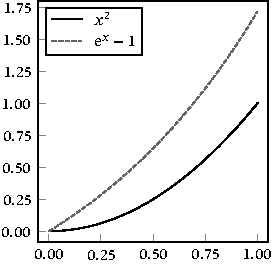
\includegraphics{speed.pdf}
  \caption{\(f(x)\)と\(g(x)\)のグラフ}
  \label{figure:speed}
\end{figure}

この理由はランダウの記号によって説明できる.まず
\[
  \abs*{\frac{g(h)}{h}} = \abs*{\frac{\napr^h-1}{h}}
  \to \abs{(\eval{(\napr^x)'}_{x=0})}
  = 1\quad(h\to 0)
\]
なので,\cref{example:bigo_ratio}から\(f(x)=\Order(x)\)(\(x\to 0\))である.
\end{example}

\section{ルンゲ現象}
関数を補間多項式で近似するときは,通過させる点(この点を\impact{標本点}\index{ひょうほんてん@標本点}という)の取り方に注意する必要がある.
\[
  f(x) = \frac{1}{1+25x^2},
  \quad x_i = -1+2\cdot\frac{i-1}{n-1}\quad(i=1,\dots,n)
\]
とおき,\(p_n(x)\)を点\((x_1,f(x_1)),\dots,(x_n,f(x_n))\)に関する補間多項式とすると,\(p_5(x)\)と\(p_9(x)\)のグラフは\cref{figure:runge}のようになる.

\begin{figure}[htbp]
  \centering
  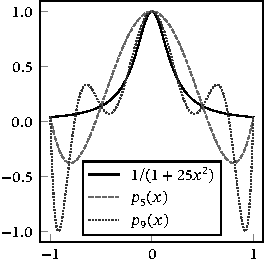
\includegraphics{runge.pdf}
  \caption{\(f(x)\)と\(n=5,9\)のときの\(p_n(x)\)}
  \label{figure:runge}
\end{figure}

\cref{figure:runge}によれば,標本点の個数\(n\)を増やすほど,\(p_n(x)\)は(特に\(x=\pm 1\)付近で著しく)\(f(x)\)からかけ離れている.
この現象を\impact{ルンゲ現象}\index{るんげげんしょう@ルンゲ現象}(Runge's phenomenon)という.

ルンゲ現象を回避するには,標本点の\(x\)座標を\impact{チェビシェフノード}\index{ちぇびしぇふのーど@チェビシェフノード}(Chebyshev nodes)である
\[
  x_i = \cos\pqty*{\frac{2i-1}{2n}\krez}\quad (i=1,\dots,n)
\]
にすると良いことが知られている\cite{horinouchi2015}.このとき,\(n=9\)の下で補間多項式\(p(x)\)は\cref{figure:chebyshev}のようになる.

\begin{figure}[htbp]
  \centering
  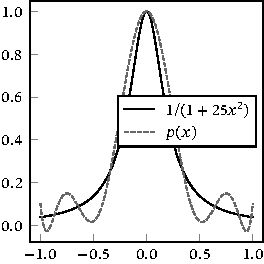
\includegraphics{chebyshev.pdf}
  \caption{チェビシェフノードを利用した補間多項式}
  \label{figure:chebyshev}
\end{figure}

\section*{演習問題}
\begin{problem}
5点\((t-2h,f(t-2h)),\dots,(t+2h,f(t+2h))\)に関する補間多項式\(p(x)\)に基づく\(f\)の数値微分を計算せよ.
また,\(f\)に適当な仮定を課して\(f'(t)=p'(t)+\Order(h^3)\)(\(h\to 0\))が成立することを示せ.
\end{problem}

\end{document}
